\documentclass[../DCM2_Verslag.tex]{subfiles}
\begin{document}


\section{Uitgevoerd onderzoek}
Er zijn drie soorten (deel)onderzoeken gedaan:\\
\-/ Wat is de maximale bandbreedte van de ESP32 bij de standaard Iperf instellingen (Baseline).\\
\-/ Welke window size geeft de hoogste bandbreedte\\
\-/ Welke package size geeft de hoogste bandbreedte\\
De paragrafen van dit hoofdstuk geven de resultaten van elk onderzoek met een korte samenvatting van de uitvoering van het onderzoek.
\clearpage
\subsection{Baseline}
In dit (deel)onderzoek is de bandbreedte onderzocht bij de standaard instellingen van Iperf. \\
De commando's gebruikt om deze resultaten te behalen zijn:\\
\begin{center}
\begin{tabular}{||l|l|l|}
   	 Testsoort & ESP32 Iperf commando & PC Iperf commando\\
   	 \hline \hline    
   	 UDP RX & iperf \-/ u \-/ s & iperf \-/ u \-/ c ESP32\_IP \\
   	 UDP TX & iperf \-/ u \-/ c PC\_IP & iperf \-/ u \-/ s \\
   	 TCP RX & iperf \-/ s & iperf \-/ c ESP32\_IP  \\
   	 TCP TX & iperf \-/ c PC\_IP & iperf \-/ s \\   	 
   	 \hline
	\end{tabular}
\end{center}
De testopstelling is onveranderd en bestaat nog steeds uit een PC, ESP32 en een WiFi accespoint.\\
Elke test is 3 keer uitgevoerd en het gemiddelde resultaat is hieronder in een tabel en grafiek uitgezet.\\
\begin{tabular}{||l|l||}
   	 Testsoort & Bandbreedte \\ & (Mbits/sec)\\
   	 \hline \hline    
   	 UDP RX & 1.07\\
   	 UDP TX & 56.83 \\
   	 TCP TX & 49.64\\
   	 TCP RX & 46.87\\
   	 \hline
	\end{tabular}
 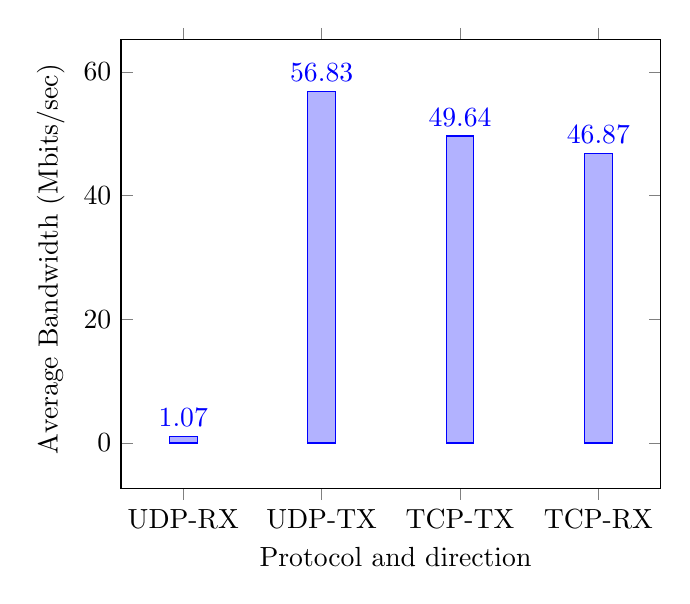
\begin{tikzpicture}[baseline=(current axis.outer west)]
\begin{axis}  
[  
    ybar,  
    enlargelimits=0.15,  
    ylabel={\ Average Bandwidth (Mbits/sec)},  
    xlabel={\ Protocol and direction},  
    symbolic x coords={UDP-RX, UDP-TX, TCP-TX, TCP-RX}, 
    xtick=data,  
    nodes near coords,
    nodes near coords align={vertical},  
]  
\addplot coordinates {(UDP-RX, 1.07) (UDP-TX, 56.83) (TCP-TX,49.64) (TCP-RX,46.87)};  
  
\end{axis}  
\end{tikzpicture} 
 \clearpage
\subsection{Window sizes}
In dit (deel)onderzoek is de bandbreedte onderzocht bij de verschillende window sizes met behulp van Iperf. \\
De commando's gebruikt om deze resultaten te behalen zijn:\\
\begin{center}
\begin{tabular}{||l|l|l|}
   	 Testsoort & ESP32 Iperf commando & PC Iperf commando\\
   	 \hline \hline    
   	 Window size (ESP32 server) & iperf \-/ s & iperf \-/ c ESP32\_IP \-/W Window\_size\\
   	 Window size (PC server) & iperf \-/ c PC\_IP & iperf \-/ s \-/W Window\_size \\
   	 \hline
	\end{tabular}
\end{center}
De testopstelling is onveranderd en bestaat nog steeds uit een PC, ESP32 en een WiFi accespoint.\\
Elke test is 3 keer uitgevoerd en de gemiddelde resultaten zijn hieronder in een tabel en grafiek uitgezet.\\
\subsubsection{Window sizes test met ESP32 als server}
Bij deze test wordt de bandbreedte gemeten met varierende window sizes waarbij de ESP32 als server en PC als client wordt gebruikt.\\
	\begin{tabular}{||l | l||}
   	 Window size(Kbytes) & Bandbreedte\\ 
   	                     & (Mbits/sec)\\
   	 \hline \hline    
   	 4 KB & 38.53  \\
   	 8 KB & 37.12  \\
   	 16 KB & 35.95 \\
   	 32 KB & 39.54  \\
   	 64 KB & 41.55  \\
   	 128 KB & 42.43  \\
   	 256 KB & 42.84  \\
   	 400 KB & 40.98 \\
   	 \hline
	\end{tabular}
	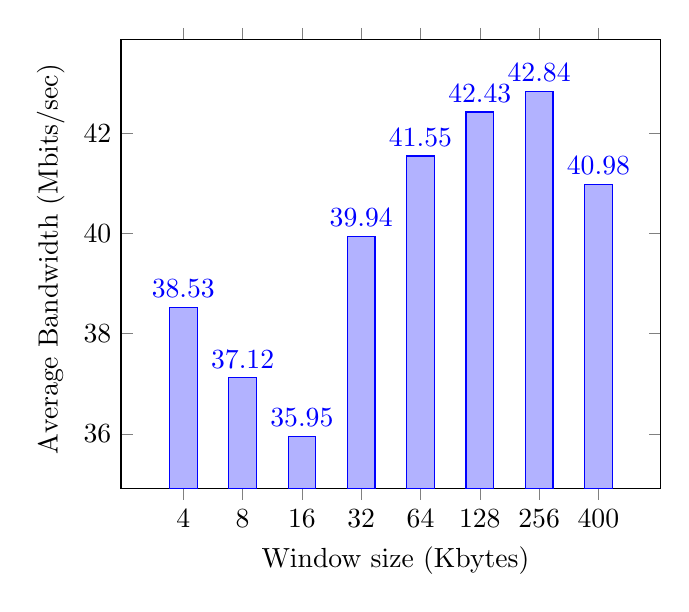
\begin{tikzpicture}[baseline=(current axis.outer east)]
	\begin{axis} [
    ybar= 5pt, 
    symbolic x coords={4,8,16,32,64,128,256,400}, 
    enlargelimits=0.15,   
    ylabel={\ Average Bandwidth (Mbits/sec)},  
    xlabel={\ Window size (Kbytes)},  
    xtick={4,8,16,32,64,128,256,400},  
    nodes near coords,
    nodes near coords align={vertical},  
   ]  
	\addplot coordinates {
    (4,38.53) 
    (8,37.12)
	(16,35.95)
    (32,39.94)
	(64, 41.55)
	(128,42.43)
	(256,42.84)
	(400,40.98)
	};
\end{axis}
\end{tikzpicture}
\clearpage
\subsubsection{Window sizes test met PC als server}
Bij deze test wordt de bandbreedte gemeten met varierende window sizes waarbij de ESP32 als client en PC als server wordt gebruikt.\\
	\begin{tabular}{||l | l||}
   	 Window size(Kbytes) & Bandbreedte\\ 
   	                     & (Mbits/sec)\\
   	 \hline \hline    
   	 4 KB & 4.8  \\
   	 8 KB & 9.32  \\
   	 16 KB & 16.18 \\
   	 32 KB & 26.56  \\
   	 64 KB & 36.76  \\
   	 128 KB & 44.49  \\
   	 256 KB & 43.66  \\
   	 400 KB & 43.9 \\
   	 \hline
	\end{tabular}
	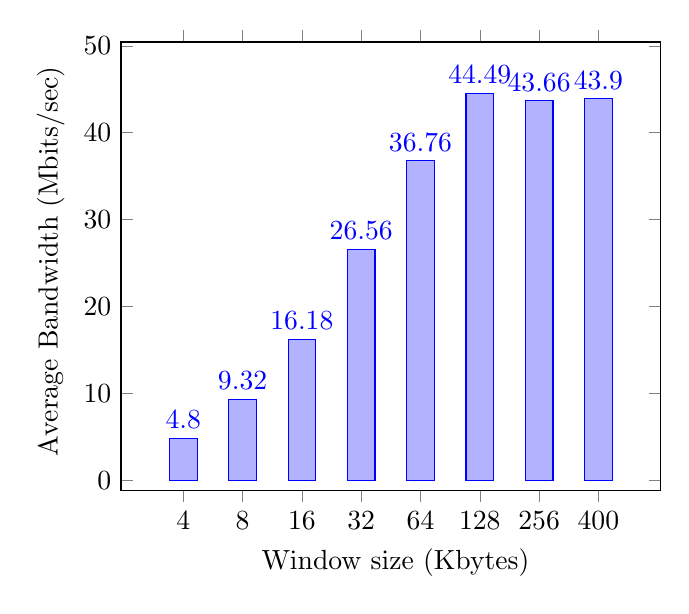
\begin{tikzpicture}[baseline=(current axis.outer east)]
	\begin{axis} [
    ybar= 5pt, 
    symbolic x coords={4,8,16,32,64,128,256,400}, 
    enlargelimits=0.15,   
    ylabel={\ Average Bandwidth (Mbits/sec)},  
    xlabel={\ Window size (Kbytes)},  
    xtick={4,8,16,32,64,128,256,400},  
    nodes near coords,
    nodes near coords align={vertical},  
   ]  
	\addplot coordinates {
    (4,4.8) 
    (8,9.32)
	(16,16.18)
    (32,26.56)
	(64,36.76)
	(128,44.49)
	(256,43.66)
	(400,43.90)
	};
\end{axis}
\end{tikzpicture}
\clearpage
\subsection{Package sizes}
In dit (deel)onderzoek is de bandbreedte onderzocht bij de verschillende package sizes met behulp van Iperf. \\
De commando's gebruikt om deze resultaten te behalen zijn:\\
\begin{center}
\begin{tabular}{||l|l|l|}
   	 Testsoort & ESP32 Iperf commando & PC Iperf commando\\
   	 \hline \hline    
   	 Window size (ESP32 server) & iperf \-/ s & iperf \-/ c ESP32\_IP \-/M MSS\_size\\
   	 Window size (PC server) & iperf \-/ c PC\_IP & iperf \-/ s \-/M MSS\_size \\
   	 \hline
	\end{tabular}
\end{center}
In de testen die uitgevoerd zijn, is de package size bepaald met behulp van de MSS grootte. MSS staat voor Max Segment Size en is het maximale formaat van het segment dat de NIC of PHY over het medium stuurt. \\
Of het ook daadwerkelijk het formaat is wat aangegeven wordt in de opties van het Iperf commando, is geen gegeven. De NIC of PHY kan afhankelijk van de fabrikant toch nog een andere MSS kiezen.\\
De testopstelling is onveranderd en bestaat nog steeds uit een PC, ESP32 en een WiFi accespoint.\\
Elke test is 3 keer uitgevoerd en de gemiddelde resultaten zijn hieronder in een tabel en grafiek uitgezet.\\
\subsubsection{Package sizes test met ESP32 als server}
Bij deze test wordt de bandbreedte gemeten met varierende package sizes waarbij de ESP32 als server en PC als client wordt gebruikt.\\
	\begin{tabular}{||l | l||}
   	 Package size(bytes) & Bandbreedte\\ 
   	                     & (Mbits/sec)\\
   	 \hline \hline    
   	 200 bytes (160 bytes MSS) &  0.0066\\
   	 400 bytes (360 bytes MSS) &  0.1\\
   	 600 bytes (560 bytes MSS) &  0.35\\
   	 800 bytes (760 bytes MSS) &  32.18\\
   	 1000 bytes (960 bytes MSS) & 34.54\\
   	 1200 bytes (1160 bytes MSS) & 35.64\\
   	 1400 bytes (1360 bytes MSS) & 40.11\\
   	 \hline
	\end{tabular}
	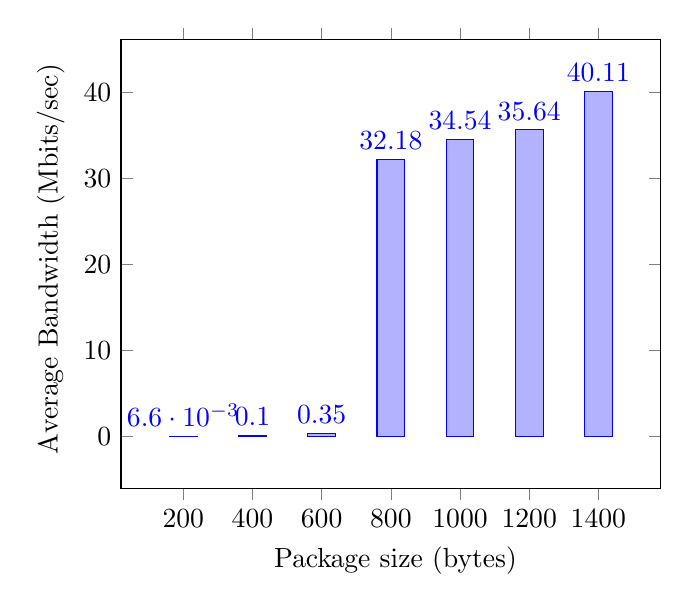
\begin{tikzpicture}[baseline=(current axis.outer east)]
	\begin{axis} [
    ybar= 5pt, 
    symbolic x coords={200,400,600,800,1000,1200,1400}, 
    enlargelimits=0.15,   
    ylabel={\ Average Bandwidth (Mbits/sec)},  
    xlabel={\ Package size (bytes)},  
    xtick={200,400,600,800,1000,1200,1400}, 
    nodes near coords,
    nodes near coords align={vertical},  
   ]  
	\addplot coordinates {
    (200, 0.0066) 
    (400, 0.1)
    (600, 0.35)
	(800, 32.18)
    (1000,34.54)
	(1200,35.64)
	(1400,40.11)
	};
\end{axis}
\end{tikzpicture}
\clearpage
\subsubsection{Package sizes test met ESP32 als client}
Bij deze test wordt de bandbreedte gemeten met varierende package sizes waarbij de ESP32 als client en PC als server wordt gebruikt.\\
	\begin{tabular}{||l | l||}
   	 Package size(bytes) & Bandbreedte\\ 
   	                     & (Mbits/sec)\\
   	 \hline \hline    
   	 200 bytes (160 bytes MSS) &  8.65\\
   	 400 bytes (360 bytes MSS) &  18.58\\
   	 600 bytes (560 bytes MSS) &  35.5\\
   	 800 bytes (760 bytes MSS) &  29.05\\
   	 1000 bytes (960 bytes MSS) & 29.02\\
   	 1200 bytes (1160 bytes MSS) & 24.79\\
   	 1400 bytes (1360 bytes MSS) & 26.97\\
   	 \hline
	\end{tabular}
	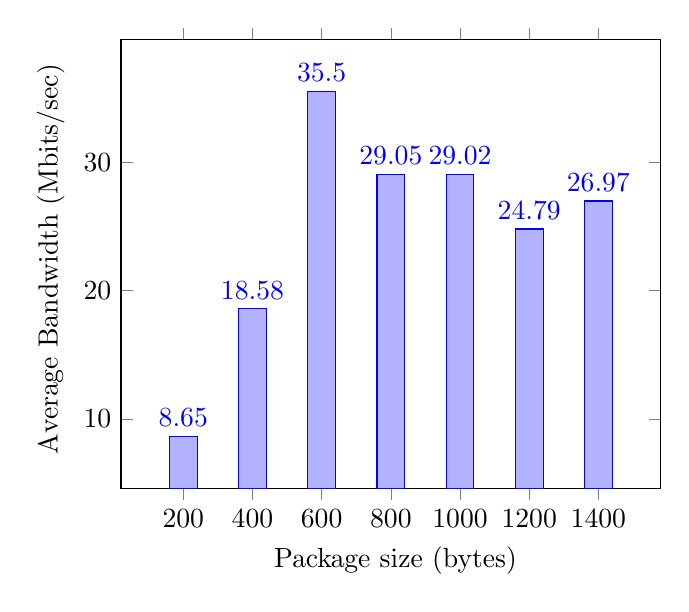
\begin{tikzpicture}[baseline=(current axis.outer east)]
	\begin{axis} [
    ybar= 5pt, 
    symbolic x coords={200,400,600,800,1000,1200,1400}, 
    enlargelimits=0.15,   
    ylabel={\ Average Bandwidth (Mbits/sec)},  
    xlabel={\ Package size (bytes)},  
    xtick={200,400,600,800,1000,1200,1400}, 
    nodes near coords,
    nodes near coords align={vertical},  
   ]  
	\addplot coordinates {
    (200,8.65) 
    (400,18.58)
    (600, 35.5)
	(800, 29.05)
    (1000,29.02)
	(1200, 24.79)
	(1400, 26.97)
	};
\end{axis}
\end{tikzpicture}


\end{document}
